\documentclass[t]{beamer}

\usepackage[brazil]{babel}
\usepackage[utf8]{inputenc}
\usepackage[T1]{fontenc}

\usepackage{listings}
\usepackage{fancyvrb}
\usepackage{color}		% Colors
\usepackage{graphicx}	% Allows including images
\usepackage{booktabs}	% Allows the use of \toprule, \midrule and \bottomrule in tables

\usepackage{fixltx2e}
\usepackage{hyperref}

\usepackage{array}
\usepackage{multirow}

\usepackage{pdfpages}
\usepackage{tikz}
\usepackage{fp}
\usepackage{xfp}
\usepackage{xparse}

\ExplSyntaxOn
\NewExpandableDocumentCommand{\fpcompare}{ m m m }
 {
  % #1 = test to perform
  % #2 = text for the true case
  % #3 = text for the false case
  \fp_compare:nTF { #1 } { #2 } { #3 }
 }
\ExplSyntaxOff

\usepackage{todonotes}

% This is necessary to perform changes into original texttt
\usepackage{textcomp}
\usepackage{upquote}
\usepackage{regexpatch}
\usepackage{xparse}

% Helps displaying correct quotes in texttt
\usepackage{csquotes}

\usepackage{natbib}
\setlength{\bibhang}{0pt}
\let\cite\citep

% Code marker colors:
\definecolor{darkgreen}{rgb}{0, 0.5, 0}
\definecolor{auburn}{rgb}{0.43, 0.21, 0.1}
\definecolor{darkspringgreen}{rgb}{0.09, 0.45, 0.27}
\definecolor{deepcarmine}{rgb}{0.66, 0.13, 0.24}
\definecolor{sapphire}{rgb}{0.03, 0.15, 0.4}
\definecolor{carmine}{rgb}{0.59, 0.0, 0.09}
\definecolor{goldenbrown}{rgb}{0.6, 0.4, 0.08}

\mode<presentation> {
	\usetheme{Madrid}
	\usecolortheme{seagull}
}

\setbeamertemplate{caption}[numbered]

\beamertemplatenavigationsymbolsempty

\lstset{
basicstyle=\ttfamily\footnotesize,
keywordstyle=\bfseries\color{darkspringgreen},
commentstyle=\itshape\color{purple!40!black},
identifierstyle=\ttfamily\footnotesize,
stringstyle=\color{auburn},
language=[AlLaTeX]TeX,
breaklines=true,
xleftmargin=.05\textwidth, 
xrightmargin=.05\textwidth,
frame=single,
tabsize=4,
escapeinside={@*}{*@},
literate=%
{á}{{\'a}}1
{à}{{\`a}}1
{ã}{{\~a}}1
{é}{{\'e}}1
{ê}{{\^e}}1
{í}{{\'i}}1
{ó}{{\'o}}1
{õ}{{\~o}}1
{ô}{{\^o}}1
{ú}{{\'u}}1
{ü}{{\"u}}1
{ç}{{\c{c}}}1
{ñ}{{\~n}}1		
}

\setbeamertemplate{footline}
    {\begin{beamercolorbox}[sep=1ex]{author in head/foot}
      \hfill\insertframenumber%
      \end{beamercolorbox}%
}

% TEXTTT
% Changes into original texttt, in order to support a more flexible textcode
\makeatletter
\def\active@text@prime{\ifin@texttt\textquotesingle\else'\fi}
\def\active@math@prime{^\bgroup\prim@s}
\newif\ifin@texttt

\regexpatchcmd{\pr@m@s}{\'}{\cA\'}{}{}
\xapptocmd{\ttfamily}{\in@texttttrue}{}{}

\begingroup\lccode`\~=`\'
\lowercase{\endgroup\protected\def~}{%
  \ifmmode
    \expandafter\active@math@prime
  \else
    \expandafter\active@text@prime
  \fi}
\AtBeginDocument{\catcode`\'=\active}

% fix \@resetactivechars not to redefine the active apostrophe
\begingroup
\obeylines\obeyspaces%
\gdef\@resetactivechars{%
\def^^M{\@activechar@info{EOL}\space}%
\def {\@activechar@info{space}\space}%
}%
\endgroup

\makeatother

\renewcommand{\ttdefault}{pcr}
\newcommand{\ownsrc}{\vspace{0.2cm} \small{Fonte: Autoria própria}}

\newcommand{\bgcolor}[3]{\colorbox{#1}{\color{#2}{#3}}}
\newcommand{\vmark}[2]{\textcolor{#1}{#2}}

% HIGHLIGHTS
\newcommand{\sel}[1]{\textbf{\texttt{\textcolor{sapphire}{#1}}}}
\newcommand{\seli}[1]{\textbf{\texttt{\textcolor{carmine}{#1}}}}
\newcommand{\selii}[1]{\textbf{\texttt{\textcolor{goldenbrown}{#1}}}}

\newcommand{\change}[1]{\textbf{\texttt{\textcolor{blue}{#1}}}}
\newcommand{\nota}[1]{\textbf{\texttt{#1}}}

% Definição da linguagem bibLatex
\lstdefinelanguage{BibTeX}{%
	keywords=[1]{@article,@book,@collectedbook,@conference,@electronic,@ieeetranbstctl,@inbook,@incollectedbook,@incollection,@injournal,@inproceedings,@manual,@mastersthesis,@misc,@patent,@periodical,@phdthesis,@preamble,@proceedings,@standard,@string,@techreport,@unpublished},
	keywords=[2]{address,annote,author,booktitle,chapter,crossref,edition,editor,howpublished,institution,journal,key,month,note,number,organization,pages,publisher,school,series,title,type,volume,year},
   comment=[l][\itshape]{@comment},
   sensitive=false,
}

%----------------------------------------------------------------------------------------
%	TITLE PAGE
%----------------------------------------------------------------------------------------

\title[\LaTeX]{\LaTeX}

\author{Giovane de Oliveira Torres}
\institute[UFPel]
{
Instituto Federal Sul-Riograndense \\
Câmpus Pelotas \\
Tecnologia em Sistemas para Internet \\
\medskip \textit{ggiovaneotorres@gmail.com} 
}
\date{7 de Novembro de 2018}

\begin{document}

\begin{frame}
\titlepage % Print the title page as the first slide
\end{frame}

% Motivaçãozinha 

\begin{frame} \frametitle{Motivação}
\begin{itemize}
	\item Alternativa para escrita de relatórios, artigos, TCCs, dentre outros documentos acadêmicos
	\item Abstrai a formatação para quem escreve o texto
	\item Referenciação de seções, figuras e bibliografia
\end{itemize}
\end{frame}

% Ferramentas
\section{Ferramentas}

\begin{frame}[fragile] \frametitle{Como começamos?}
\begin{itemize}
	\item \textit{Software} essencial para construção de documentos em Latex
	\begin{itemize}
		\item Miktex\footnote{\url{https://miktex.org/}}
		\begin{itemize}
			\item Comumente utilizado no Windows
		\end{itemize}
		\item Texlive\footnote{\url{https://www.tug.org/texlive/}}
		\begin{itemize}
			\item Comumente utilizado em sistemas baseados em Linux
		\end{itemize}
	\end{itemize}
\end{itemize}
\end{frame}

\begin{frame}[fragile] \frametitle{Como começamos?}
\begin{itemize}
	\item Tendo um dos programas citados, podemos utilizar \textbf{qualquer} editor de texto
	\begin{itemize}
		\item Basta saber como compilar o arquivo fonte
	\end{itemize}
	\item Porém, existem alternativas
\end{itemize}
\end{frame}

\begin{frame}[fragile] \frametitle{IDEs}
\begin{itemize}
	\item Podemos utilizar IDEs que facilitam um pouco o trabalho
	\item IDEs contam com \textit{syntax highlighting}, métodos de compilação em um clique, facilidades para utilizar os comandos a serem vistos, dentre outros
	\begin{itemize}
		\item Texmaker~\footnote{\url{http://www.xm1math.net/texmaker/}} (recomendado)
		\begin{itemize}
			\item Funciona em Windows, Linux e MacOsX
			\item \textit{Cross-platform}
		\end{itemize}
		\item Texworks~\footnote{\url{http://www.tug.org/texworks/}}
		\item Kile~\footnote{\url{https://kile.sourceforge.io/}}
	\end{itemize}
\end{itemize}
\end{frame}

\begin{frame}[fragile] \frametitle{Via web}
\begin{itemize}
	\item Podemos usar editores web
	\item Apresentam suporte à escrita colaborativa
	\begin{itemize}
		\item Overleaf~\footnote{\url{https://www.overleaf.com/}}
		\item ShareLaTeX~\footnote{\url{https://www.sharelatex.com/}}
	\end{itemize}
\end{itemize}
\end{frame}
% Ambiente
\section{Ambiente}

\begin{frame} \frametitle{Iniciando um documento no formato .tex}
\begin{itemize}
	\item Criar um arquivo .tex
	\item Deve ser necessário alguns comandos
\end{itemize}
\end{frame}

\begin{frame}[fragile] \frametitle{Iniciando um documento no formato .tex}
\begin{figure}[!t]
\begin{lstlisting}
\documentclass{article}

\begin{document}
	Ola mundo
\end{document}
\end{lstlisting}
\end{figure}
\end{frame}

\begin{frame}[fragile] \frametitle{Iniciando um documento no formato .tex}
\begin{figure}[!t]
\begin{lstlisting}
@*\sel{$\backslash$documentclass\{article\}}*@

\begin{document}
	Ola mundo
\end{document}
\end{lstlisting}
\end{figure}

\begin{itemize}
	\item \sel{$\backslash$documentclass\{article\}}
	\begin{itemize}
		\item Define a classe de documento que será utilizada
		\item \texttt{article}: Artigo
		\item Existem diversas opções que permite diferentes formatos de documentos
	\end{itemize}
\end{itemize}

\end{frame}

% Exemplos de documentos...

\begin{frame}[fragile] \frametitle{Iniciando um documento no formato .tex}
\begin{figure}[!t]
\begin{lstlisting}
\documentclass{article}

@*\sel{$\backslash$begin\{document\}}*@
	Ola mundo
@*\sel{$\backslash$end\{document\}}*@
\end{lstlisting}
\end{figure}

\begin{itemize}
	\item \sel{$\backslash$begin\{document\}} e \sel{$\backslash$end\{document\}}
	\begin{itemize}
		\item Delimita o escopo de conteúdo do documento
		\begin{itemize}
			\item Também chamado de corpo do documento
		\end{itemize}
		\item O que vem antes de \texttt{$\backslash$begin\{document\}} é chamado de \textbf{preâmbulo} do documento
	\end{itemize}
\end{itemize}
\end{frame}

\begin{frame} \frametitle{Preâmbulo do documento}
\begin{itemize}
	\item Primeira metade de um arquivo .tex
	\begin{itemize}
		\item \textbf{Sempre} antes do texto que irá compor o documento
	\end{itemize}
	\item Múltiplas funcionalidades
	\begin{itemize}
		\item Tipo de documento
		\item Informações para formatar o documento corretamente
		\item Carregamento de pacotes que auxiliam para algumas especificidades
	\end{itemize}
\end{itemize}
\end{frame}

\begin{frame} \frametitle{Corpo do documento}
\begin{itemize}
	\item Segunda metade do arquivo .tex
	\item Contém todas as informações referentes a conteúdo do documento
	\begin{itemize}
		\item Texto bruto
		\item Comandos para formatação de texto
		\item Inserção de elementos adicionais
		\begin{itemize}
			\item Figuras, tabelas, fórmulas matemáticas, \ldots
		\end{itemize}
	\end{itemize}
\end{itemize}
\end{frame}

\begin{frame} \frametitle{Localidade}
\begin{itemize}
	\item Por padrão, o~LaTeX~por si só não é suficiente
	\item Precisamos estabelecer a localidade para a escrita correta de textos
	\begin{itemize}
		\item Textos em português: Apresetam caracteres com acentuação (ã, ê, í, etc.)
	\end{itemize}
\end{itemize}
\end{frame}

\begin{frame} \frametitle{Localidade}
\begin{itemize}
	\item Adaptar o LaTeX~para a localidade que desejamos
	\begin{itemize}
		\item Suporte a diversas linguagens espalhadas pelo globo
	\end{itemize}
	\item Modificar para o LaTeX conseguir interpretar os acentos corretamente -- além de alterar a localidade para português brasileiro.
	\begin{itemize}
		\item \textbf{Preâmbulo} do documento
	\end{itemize}
\end{itemize}
\end{frame}

\begin{frame}[fragile] \frametitle{Localidade}
\begin{figure}[!t]
\begin{lstlisting}
\documentclass{article}

@*\sel{$\backslash$usepackage[brazil]\{babel\}}*@		% Comando para pôr a localidade português brasileiro 
\usepackage[utf8]{inputenc} 	% Comando para reconhecer entradas utilizando a codificação UTF-8

\begin{document}
(@*\ldots*@)
\end{lstlisting}
\end{figure}

\begin{itemize}
	\item \sel{$\backslash$usepackage[brazil]\{babel\}}
	\begin{itemize}
		\item Datas e palavras fornecidas pela formatação do LaTeX~são traduzidas para português brasileiro
		\item Se desejável, pode-se trocar a opção entre colchetes para a linguagem que quiser
		\begin{itemize}
			\item \texttt{english}, \texttt{spanish}, \ldots
		\end{itemize}
	\end{itemize}
\end{itemize}
\end{frame}

\begin{frame}[fragile] \frametitle{Localidade}
\begin{figure}[!t]
\begin{lstlisting}
\documentclass{article}

\usepackage[brazil]{babel}		% Comando para pôr a localidade português brasileiro
@*\sel{$\backslash$usepackage[utf8]\{inputenc\}}*@ 	% Comando para reconhecer entradas utilizando a codificação UTF-8

\begin{document}
(@*\ldots*@)
\end{lstlisting}
\end{figure}

\begin{itemize}
	\item \sel{$\backslash$usepackage[utf8]\{inputenc\}}
	\begin{itemize}
		\item Mostra corretamente caracteres com acento, cedilha, dentre outros
		\item Tecnicamente, faz com que a codificação lida como entrada pelo LaTeX seja UTF-8, a qual tem suporte a vários caracteres (inclusos os utilizados no português)
	\end{itemize}
\end{itemize}
\end{frame}

\begin{frame}[fragile] \frametitle{Localidade}
\begin{figure}[!t]
\begin{lstlisting}
\documentclass{article}

\usepackage[brazil]{babel}		% Comando para pôr a localidade português brasileiro
@*\sel{$\backslash$usepackage[utf8]\{inputenc\}}*@	% Comando para reconhecer entradas utilizando a codificação UTF-8

\begin{document}
(@*\ldots*@)
\end{lstlisting}
\end{figure}

\begin{itemize}
	\item \sel{$\backslash$usepackage[utf8]\{inputenc\}}
	\begin{itemize}
		\item Podem ser usados outros tipos de codificação, como \texttt{latin1} em vez de \texttt{utf8}, a qual corresponde à codificação ISO 8859-1
		\item \textbf{Recomendação pessoal}: Usar UTF-8
	\end{itemize}
\end{itemize}
\end{frame}
% Uso de classes
\section{Classes}

\begin{frame} \frametitle{Classes}
\begin{itemize}
	\item Para um arquivo ser formatado corretamente, faz-se uso de classes
	\item Algumas classes pré-definidas
	\begin{itemize}
		\item \texttt{article, book}, \ldots
	\end{itemize}
	\item Classes construídas por usuários
	\begin{itemize}
		\item Arquivo .cls
	\end{itemize}
\end{itemize}
\end{frame}

\begin{frame} \frametitle{Arquivo .cls}
\begin{itemize}
	\item Define uma classe de arquivo a qual representa uma formatação definida
	\item Utiliza a linguagem TeX para desenvolver
	\begin{itemize}
		\item Linguagem complexa e de difícil entendimento
	\end{itemize}
\end{itemize}
\end{frame}

\begin{frame} \frametitle{Classe do TCC do TSI-IFSul}
\begin{itemize}
	\item \textbf{Caso de exemplo:} Classe do documento de TCC do TSI-IFSul Campus Pelotas
	\begin{itemize}
		\item Segue a mesma formatação do modelo de documento fornecido em .doc
	\end{itemize}
	\item Disponível em um repositório do GitHub:
	\begin{itemize}
		\item \url{https://github.com/gdotorres/tsi-ifsul-tcc}
	\end{itemize}
\end{itemize}
\end{frame}

\begin{frame} \frametitle{Classe do TCC do TSI-IFSul}
\begin{itemize}
	\item Arquivo \textbf{textsi.cls}: Define a formatação geral do documento
	\begin{itemize}
		\item Margens, fonte, espaçamento, \ldots
		\item Define usos de alguns pacotes
		\begin{itemize}
			\item Requeridos para o desenvolvimento desta classe
		\end{itemize}
		\item Desenvolvido na linguagem TeX
	\end{itemize}
	\item Arquivo \textbf{exemplo-tcc.tex}: Pacotes adicionais e corpo do documento
	\begin{itemize}
		\item Focaremos principalmente neste arquivo
	\end{itemize}
	\item Arquivo \textbf{exemplo-tcc.bib}: Referências bibliográficas
	\begin{itemize}
		\item Será visto com mais detalhes adiante
	\end{itemize}
\end{itemize}
\end{frame}

\begin{frame} \frametitle{Classe do TCC do TSI-IFSul -- Entendimento}
\begin{itemize}
	\item \textbf{exemplo-tcc.tex} é composto de conteúdo com comentários indicando para que serve cada linha ou conjunto de linhas de comando
\end{itemize}
\end{frame}

\begin{frame}[fragile] \frametitle{Comentários?}

\begin{lstlisting}
@*\sel{\% Começo de um documento .tex}*@
\documentclass{article} 
(...)
\end{lstlisting}

\begin{itemize}
	\item Estamos utilizando uma linguagem de programação para descrever nosso documento
	\item Como linguagem de programação, ela fornece meio para comentários
	\begin{itemize}
		\item Utilizamos o caractere \%
		\item Somente uma nova linha no código para desfazer o comentário
		\item \textbf{Não} existe comentário em bloco
	\end{itemize}
\end{itemize}
\end{frame}
% Inserção de texto
\section{Texto}

\begin{frame}[fragile] \frametitle{Inserção de texto}
\begin{itemize}
	\item Para inserir texto, é extremamente simples
	\item Basta digitá-lo dentro do corpo de documento
	\item Entre \texttt{$\backslash$begin\{document\}} e \texttt{$\backslash$end\{document\}}
\end{itemize}
\end{frame}

\begin{frame}[fragile] \frametitle{Inserção de texto}
\begin{figure}[!t]
\begin{lstlisting}
(@*\ldots*@)
\begin{document}
(@*\ldots*@)
	Escrever um texto em LaTeX é simples como testar todos os caracteres como "The quick brown fox jumps over the lazy dog".
(@*\ldots*@)
\end{document}
\end{lstlisting}
\end{figure}
\end{frame}

\begin{frame}[fragile] \frametitle{Inserção de texto}
\begin{itemize}
	\item O próprio LaTeX acha o melhor meio de fazer o texto caber dentro das margens
	\begin{itemize}
		\item Utiliza o espaçamento adequadamente
		\item Consegue fazer a quebra de palavras utilizando separação de sílabas para melhor disposição do texto em uma linha
	\end{itemize}
	\item Porém um texto pode apresentar outras características
	\begin{itemize}
		\item Como fazer um novo parágrafo?
		\item Uma nova linha?
	\end{itemize}
\end{itemize}
\end{frame}

\begin{frame} \frametitle{Parágrafos}
\begin{itemize}
	\item Diferentes métodos para adição de parágrafos
	\begin{enumerate}
		\item Inserção de uma linha em branco entre dois parágrafos.
		\item Comando \texttt{\textbackslash{}par}
	\end{enumerate}
\end{itemize}
\end{frame}

\begin{frame}[fragile] \frametitle{Parágrafos}
\begin{figure}[!t]
\begin{lstlisting}
(@*\ldots*@)
\begin{document}
(@*\ldots*@)
	Escrever um texto em LaTeX é simples como testar todos os caracteres como "The quick brown fox jumps over the lazy dog".

	Existe uma linha em branco acima da primeira linha, logo esta linha será um novo parágrafo.
	Note que esta frase não aparece em um novo parágrafo, já que não existe uma linha em branco entre a frase anterior e esta. \par Já esta frase irá aparecer como um novo parágrafo, dado que estamos inserindo o comando para fazê-lo.
(@*\ldots*@)
\end{document}
\end{lstlisting}
\end{figure}
\end{frame}

\begin{frame}[fragile] \frametitle{Nova linha}
\begin{itemize}
	\item Diferentes métodos para adição de uma nova linha
	\begin{enumerate}
		\item Método usual: comando $\backslash\backslash$
		\item Método alternativo: comando $\backslash$newline
	\end{enumerate}
\end{itemize}
\end{frame}

\begin{frame}[fragile] \frametitle{Inserção de texto}
\begin{figure}[!t]
\begin{lstlisting}
(@*\ldots*@)
\begin{document}
(@*\ldots*@)
	Escrever um texto em LaTeX é simples como testar todos os caracteres como "The quick brown fox jumps over the lazy dog". \\ Existem duas contrabarras logo após a primeira frase, logo esta frase aparece em uma nova linha.
(@*\ldots*@)
\end{document}
\end{lstlisting}
\end{figure}

\begin{itemize}
	\item Nova linha \textbf{não é} novo parágrafo
	\begin{itemize}
		\item Parágrafo tem o recuo à direita em relação a uma nova linha
	\end{itemize}
\end{itemize}
\end{frame}

	
% Formatação básica de texto
\section{Formatação básica}

\begin{frame}[fragile] \frametitle{Formatação básica}
\begin{itemize}
	\item Somente texto cru não faz muita coisa
	\item Vários elementos de formatação também se fazem presentes no LaTeX
\end{itemize}
\end{frame}

\begin{frame}[fragile] \frametitle{Negrito, itálico e sublinhado}
\begin{figure}[!t]
\begin{lstlisting}
Eis que você está digitando um texto e deseja fazer um @*\sel{\textbackslash{}textbf\{destaque\}}*@. A palavra "destaque" da frase anterior irá aparecer em negrito.
\end{lstlisting}
\end{figure}

\begin{itemize}
	\item \sel{$\backslash$textbf\{texto\}}
	\begin{itemize}
		\item Formata texto em negrito
	\end{itemize}
\end{itemize}
\end{frame}

\begin{frame}[fragile] \frametitle{Negrito, itálico e sublinhado}
\begin{figure}[!t]
\begin{lstlisting}
Usualmente, utiliza-se texto em itálico para destacar palavras estrangeiras, como @*\sel{$\backslash$textit\{smartphone\}}*@.
\end{lstlisting}
\end{figure}

\begin{itemize}
	\item \sel{$\backslash$textit\{texto\}}
	\begin{itemize}
		\item Formata texto em itálico
	\end{itemize}
\end{itemize}
\end{frame}

\begin{frame}[fragile] \frametitle{Negrito, itálico e sublinhado}
\begin{figure}[!t]
\begin{lstlisting}
E dá pra @*\sel{$\backslash$underline\{deixar elementos sublinhados\}}*@.
\end{lstlisting}
\end{figure}

\begin{itemize}
	\item \sel{$\backslash$underline\{texto\}}
	\begin{itemize}
		\item Formata texto em sublinhado
	\end{itemize}
\end{itemize}
\end{frame}

\begin{frame}[fragile] \frametitle{Negrito, itálico e sublinhado}
\begin{figure}[!t]
\begin{lstlisting}
E o que acontece se fizermos uma \textbf{\textit{salada}} \textit{\underline{mista}}?
\end{lstlisting}
\end{figure}

\begin{itemize}
	\item Quando fazemos $\backslash$\texttt{comando}, estamos invocando um comando.
	\item Podemos invocar comandos aninhados
	\begin{itemize}
		\item \texttt{$\backslash$comando1\{$\backslash$comando2\{texto\}\}}
	\end{itemize}
	\item Primeiro destaque: Negrito e itálico
	\item Segundo destaque: Itálico e sublinhado
\end{itemize}
\end{frame}
% Seções, subseções e etc..
\section{Secionamento}

\begin{frame}[fragile] \frametitle{Secionamento}
\begin{itemize}
	\item A fim de promover uma organização melhor no texto, utilizamos seções
	\item Estas seções são \textbf{usualmente} numeradas
	\item Caso de exemplo: \textbf{Template do TCC-TSI}
	\begin{itemize}
		\item Cinco níveis de seção
		\item Seção primária (1), seção secundária (1.1), \ldots, seção quinária (1.1.1.1.1)
	\end{itemize}
	\item Numeração das seções: feita \textbf{automaticamente}
\end{itemize}
\end{frame}

\begin{frame}[fragile] \frametitle{Secionamento}
\begin{table}[!t]
	\centering
	\caption{Tipo de seção e seu respectivo comando para o template do TCC do TSI}	
	\begin{tabular}{l|l}
	\hline
		\textbf{Nível da seção} & \textbf{Comando}                      \\ \hline
		Primária                & \texttt{\textbackslash{}chapter\{nome\}}       \\ \hline
		Secundária              & \texttt{\textbackslash{}section\{nome\}}       \\ \hline
		Terciária               & \texttt{\textbackslash{}subsection\{nome\}}    \\ \hline
		Quaternária             & \texttt{\textbackslash{}subsubsection\{nome\}} \\ \hline
		Quinária                & \texttt{\textbackslash{}paragraph\{nome\}}     \\ \hline
	\end{tabular}
	\\ \vspace{0.3cm} \ownsrc
\end{table}

\begin{itemize}
	\item As normas do IFSul nos restringem a no máximo seções quinárias
	\item Usualmente estes comandos são redefinidos nas classes utilizadas
\end{itemize}
\end{frame}

\begin{frame}[fragile] \frametitle{Secionamento não numerado}
\begin{itemize}
	\item Eventualmente, pode-se haver a necessidade de estruturar uma seção no documento não numerada
	\item Para isto, fazemos o uso do caractere \text{asterisco} (*) para tal fim
	\begin{itemize}
		\item Exemplo: \texttt{\textbackslash{}section*\{seção não numerada\}}
	\end{itemize}
\end{itemize}
\end{frame}

\begin{frame}[fragile] \frametitle{Secionamento (outras informações)}
\begin{itemize}
	\item Outras classes de documentos podem definir diferentes estilos de secionamento
	\item Dentro da linguagem Latex são fornecidos até 7 níveis de secionamento
\end{itemize}
\end{frame}

\begin{frame}[fragile] \frametitle{Secionamento (outras informações)}
\begin{table}[!t]
	\centering
	\caption{Tipo de seção e seu respectivo comando para o \textit{template} do TCC do TSI}	
	\begin{tabular}{l|l}
	\hline
		\textbf{Nível da seção} & \textbf{Comando}									\\ \hline
		Primária				& \texttt{\textbackslash{}part\{nome\}}				\\ \hline
		Secundária				& \texttt{\textbackslash{}chapter\{nome\}}			\\ \hline
		Terciária				& \texttt{\textbackslash{}section\{nome\}}			\\ \hline
		Quaternária				& \texttt{\textbackslash{}subsection\{nome\}}		\\ \hline
		Quinária				& \texttt{\textbackslash{}subsubsection\{nome\}}	\\ \hline
		Senária					& \texttt{\textbackslash{}paragraph\{nome\}}		\\ \hline
		Setenária				& \texttt{\textbackslash{}subparagraph\{nome\}}		\\ \hline
	\end{tabular}
	\\ \vspace{0.3cm} \ownsrc
\end{table}

\begin{itemize}
	\item Se realmente quiséssemos ir a fundo, podíamos definir outros comandos para estabelecer \textbf{mais níveis de secionamento}
\end{itemize}
\end{frame}

\begin{frame}[fragile] \frametitle{Referência à seções}
\begin{itemize}
	\item Eventualmente, podemos chegar a um ponto que precisamos fazer referência à uma determinada seção
	\item Exemplo clássico: Dentro da introdução de um TCC, falamos sobre como as demais seções estão organizadas no documento.
	\item Esta referenciação pode ser feita de maneira \textbf{automática}
	\item Utilizaremos um par de comandos para tal fim: \texttt{label} e \texttt{ref}
\end{itemize}
\end{frame}

\begin{frame}[fragile] \frametitle{Referência à seções}
\begin{figure}[!t]
\caption{Exemplo de rotulação e referenciação de seções}
\begin{lstlisting}
	\section{Laranjas} @*\sel{\textbackslash{}label\{s:laranjas\}}*@
	Laranja é laranja por causa da cor laranja ou por causa da fruta laranja?

	\section{Maracujás} @*\sel{\textbackslash{}label\{s:maracujas\}}*@
	Uma questão foi feita na Seção~\ref{s:laranjas}. Os maracujás tem a cor amarela.
\end{document}
\end{lstlisting}
\ownsrc
\end{figure}

\begin{itemize}
	\item \sel{\textbackslash{}label\{nome do rótulo\}}
	\begin{itemize}
		\item Rotula um elemento em Latex. Neste caso, estamos utilizando para uma \texttt{section}
	\end{itemize}
\end{itemize}
\end{frame}

\begin{frame}[fragile] \frametitle{Referência à seções}
\begin{figure}[!t]
\caption{Exemplo de rotulação e referenciação de seções}
\begin{lstlisting}
\section{Laranjas} \label{s:laranjas}
Laranja é laranja por causa da cor laranja ou por causa da fruta laranja?

\section{Maracujás} \label{s:maracujas}
Uma questão foi feita na Seção~@*\sel{\textbackslash{}ref\{s:laranjas\}}*@. Os maracujás tem a cor amarela.
\end{document}
\end{lstlisting}
\ownsrc
\end{figure}

\begin{itemize}
	\item \sel{\textbackslash{}ref\{nome do rótulo\}}
	\begin{itemize}
		\item Referencia um elemento em Latex previamente rotulado. O Latex encarrega-se de mostrar a numeração (neste caso) da seção corretamente
	\end{itemize}
\end{itemize}
\end{frame}
% Estruturas de listas..
\section{Estruturas de Listas}

\begin{frame}[fragile] \frametitle{Estruturas de Listas}
\begin{itemize}
	\item Em alguns casos podemos fazer uso de estruturas de listas para enumerar uma sequência de itens
	\item Algo como está sendo visualizado nesta apresentação
	\item Existem três tipos de estruturas de listas
	\begin{itemize}
		\item Não numeradas
		\item Enumeradas
		\item Descritivas
	\end{itemize}
\end{itemize}
\end{frame}

\begin{frame}[fragile] \frametitle{Listas não numeradas}
\begin{figure}[!t]
\begin{lstlisting}
@*\sel{\textbackslash{}begin\{itemize\}}*@
	\item Um item
	\item Outro item
@*\sel{\textbackslash{}end\{itemize\}}*@
\end{lstlisting}
\end{figure}

\begin{itemize}
	\item \sel{\textbackslash{}begin\{itemize\}} e \sel{\textbackslash{}end\{itemize\}}
	\begin{itemize}
		\item Denomina um \textbf{ambiente} de nome \texttt{itemize}, o qual permite construir listas não numeradas
		\item Todo tipo de comando onde for utilizado neste estilo (\texttt{begin} e \texttt{end}) é chamado de ambiente em LaTeX
	\end{itemize}
\end{itemize}
\end{frame}

\begin{frame}[fragile] \frametitle{Listas não numeradas}
\begin{figure}[!t]
\begin{lstlisting}
\begin{itemize}
	@*\sel{\textbackslash{}item}*@ Um item
	@*\sel{\textbackslash{}item}*@ Outro item
\end{itemize}
\end{lstlisting}
\end{figure}

\begin{itemize}
	\item \sel{\textbackslash{}item}
	\begin{itemize}
		\item Determina um item de uma lista não numerada
		\item Este comando \textbf{deve} estar dentro de um ambiente que permite construir listas! (Ex: \texttt{itemize})
	\end{itemize}
\end{itemize}
\end{frame}

\begin{frame}[fragile] \frametitle{Listas enumeradas}
\begin{figure}[!t]
\begin{lstlisting}
@*\sel{\textbackslash{}begin\{enumerate\}}*@
	\item Primeiro item enumerado
	\item Segundo item enumerado
@*\sel{\textbackslash{}end\{enumerate\}}*@
\end{lstlisting}
\end{figure}

\begin{itemize}
	\item \sel{\textbackslash{}begin\{enumerate\}} e \sel{\textbackslash{}end\{enumerate\}}
	\begin{itemize}
		\item Denomina um ambiente de nome \texttt{enumerate}, o qual permite construir listas enumeradas
	\end{itemize}
\end{itemize}
\end{frame}

\begin{frame}[fragile] \frametitle{Listas enumeradas}
\begin{figure}[!t]
\begin{lstlisting}
\begin{enumerate}
	@*\sel{\textbackslash{}item}*@ Um item
	@*\sel{\textbackslash{}item}*@ Outro item
\end{enumerate}
\end{lstlisting}
\end{figure}

\begin{itemize}
	\item \sel{\textbackslash{}item}
	\begin{itemize}
		\item Determina um item de uma lista enumerada
		\begin{itemize}
			\item Neste caso é enumerada porque está \textbf{dentro do ambiente} \texttt{enumerate}
		\end{itemize}
		\item O LaTeX efetua a numeração da lista automaticamente
	\end{itemize}
\end{itemize}
\end{frame}

\begin{frame}[fragile] \frametitle{Listas enumeradas manipuladas}

\begin{itemize}
	\item A priori, temos listas com números
	\item Podemos ir além
	\item Uso de um pacote \texttt{enumitem}
	\begin{itemize}
		\item \texttt{\textbackslash{}usepackage\{enumitem\}}
		\item Permite fazer manipulação nas listas de modo a permitir listas ordenadas por caractere (a, b, \ldots), números romanos (i, ii, \ldots), dentre outros
	\end{itemize}
\end{itemize}
\end{frame}

\begin{frame}[fragile] \frametitle{Listas enumeradas manipuladas}
\begin{figure}[!t]
\begin{lstlisting}
(@*\ldots*@)
\usepackage{enumitem}
(@*\ldots*@)
\begin{document}
(@*\ldots*@)
\begin{enumerate}@*\sel{[label=\textbackslash{}roman*]}*@
	\item Um item
	\item Outro item
\end{enumerate}
\end{lstlisting}
\end{figure}

\begin{itemize}
	\item \sel{[label=formato]}
	\begin{itemize}
		\item Determina que uma lista enumerada utilize um determinado formato
		\item Neste caso, estamos utilizando \textbackslash{}roman*, o qual formata os itens de uma lista do tipo \texttt{enumerate} para números romanos
	\end{itemize}
\end{itemize}
\end{frame}

\begin{frame}[fragile] \frametitle{Listas enumeradas manipuladas}
\begin{itemize}
	\item Argumento para formatação de lista enumerada é opcional
	\begin{itemize}
		\item Qualquer argumento que vier dentro de colchetes é considerado pela linguagem do LaTeX como argumento opcional
	\end{itemize}
	\item Se nada é passado para \texttt{\textbackslash{}begin\{enumerate\}} o padrão é utilizado (lista enumerada numericamente)
\end{itemize}
\end{frame}

\begin{frame}[fragile] \frametitle{Formatos de listas enumeradas}
\begin{table}[!h]
\centering
\begin{tabular}{l|l}		
\hline
	\textbf{Comando}       & \textbf{Formato} \\ \hline
	\textbackslash{}alph   & a. b. c.         \\ \hline
	\textbackslash{}Alph   & A. B. C          \\ \hline
	\textbackslash{}arabic & 1. 2. 3.         \\ \hline
	\textbackslash{}roman  & i. ii. iii.      \\ \hline
	\textbackslash{}Roman  & I. II. III       \\ \hline
\end{tabular}
\end{table}
\end{frame}

\begin{frame}[fragile] \frametitle{Listas descritivas}
\begin{figure}[!t]
\begin{lstlisting}
@*\sel{\textbackslash{}begin\{description\}}*@
	\item [Banana] Uma fruta
	\item [Maçã] Outra fruta
@*\sel{\textbackslash{}end\{description\}}*@
\end{lstlisting}
\end{figure}

\begin{itemize}
	\item \sel{\textbackslash{}begin\{description\}} e \sel{\textbackslash{}end\{description\}}
	\begin{itemize}
		\item Denomina um ambiente de nome \texttt{description}, o qual permite construir listas descritivas
	\end{itemize}
\end{itemize}
\end{frame}

\begin{frame}[fragile] \frametitle{Listas descritivas}
\begin{figure}[!t]
\begin{lstlisting}
\begin{description}
	@*\sel{\textbackslash{}item [Banana]}*@ Uma fruta
	@*\sel{\textbackslash{}item [Maçã]}*@ Outra fruta
\begin{description}
\end{lstlisting}
\end{figure}

\begin{itemize}
	\item \sel{\textbackslash{}item}
	\begin{itemize}
		\item Determina um item de uma lista descritiva
		\begin{itemize}
			\item Dentro dos colchetes vai a descrição de um item
			\item Comumente formatado em negrito
		\end{itemize}
	\end{itemize}
\end{itemize}
\end{frame}

\begin{frame}[fragile] \frametitle{\textit{Mix} de listas}
\begin{figure}[!t]
\begin{lstlisting}
\begin{itemize}
	\item Um item não numerado
	\begin{enumerate}
		\item Item enumerado-x
		\begin{enumerate}
			\item Item enumerado-y
		\end{enumerate}
	\end{enumerate}
\end{itemize}
\end{lstlisting}
\end{figure}

\begin{itemize}
	\item Podemos inserir listas dentro de listas
	\item Somente deve-se tomar cuidado em que nível estamos ao adicionar um item
\end{itemize}
\end{frame}
% Tabelas..
\section{Tabelas}

\begin{frame}[fragile] \frametitle{Tabelas}
\begin{itemize}
	\item Comumente utilizamos uma tabela para fazer a sumarização de algumas informações
	\begin{itemize}
		\item Comparar informações
		\item Mostra de dados
	\end{itemize}
	\item Um elemento não tão simples de ser inserido em LaTeX
\end{itemize}
\end{frame}

\begin{frame}[fragile] \frametitle{Tabelas}
\begin{figure}[!t]
\begin{lstlisting}
\begin{table}[!h]
\centering
\caption{legenda}
	\begin{tabular}{|c|c|} \hline
		a & b \\ \hline
		c & d \\ \hline
	\end{tabular}
\source{fonte}
\end{table}
\end{lstlisting}
\end{figure}
\begin{table}[!h]
\centering
\begin{tabular}{|c|c|} \hline
	a & b \\ \hline
	c & d \\ \hline
\end{tabular}
\end{table}
\end{frame}

\begin{frame}[fragile] \frametitle{O ambiente \texttt{table}}
\vspace{-0.5cm}
\begin{figure}[!t]
\begin{lstlisting}
@*\sel{\textbackslash{}begin\{table\}[!h]}*@
\centering
\caption{legenda}
	\begin{tabular}{|c|c|} \hline
		a & b \\ \hline
		c & d \\ \hline
	\end{tabular}
\source{fonte}
@*\sel{\textbackslash{}end\{table\}}*@
\end{lstlisting}
\end{figure}

\begin{itemize}
	\item \sel{\textbackslash{}begin\{table\}} e \sel{\textbackslash{}end\{table\}}
	\begin{itemize}
		\item Define um ambiente de tabela
		\begin{itemize}
			\item Em especial, elementos como tabela e figura são chamados no LaTeX de \textit{floats}
		\end{itemize}
		\item Pode ter como argumento opcional o \textbf{posicionamento} do \textit{float} dentro do documento
	\end{itemize}
\end{itemize}
\end{frame}

\begin{frame}[fragile] \frametitle{Posicionamento de \textit{floats}}
\begin{itemize}
	\item Definido logo após um comando \texttt{\textbackslash{}begin\{"float"\}}
	\begin{itemize}
		\item Exemplo: \texttt{\textbackslash{}begin\{table\}[!h]}
	\end{itemize}
	\item Indica um ou mais possíveis posicionamentos do \textit{float} no LaTeX
\end{itemize}

\begin{table}[!t]
\label{tab:posicaofloats}
\begin{tabular}{c|p{7.5cm}} \hline
\textbf{Caractere} & \multicolumn{1}{c}{\textbf{Significado}} \\ \hline
h & Posiciona "aqui", sendo colocado aproximadamente no mesmo ponto que ocorre no texto.            \\ \hline
t & Posiciona ao topo da página             \\ \hline
b & Posiciona na base da página             \\ \hline
p & Insere em uma página especial somente para floats     \\ \hline
! & Sobrepõe os parâmetros internos que o LaTeX utiliza para determinar "boas"~posições para floats \\ \hline
\end{tabular}
\end{table}
\end{frame}

\begin{frame}[fragile,label={slide:floatcentering}] \frametitle{Centralização de \textit{floats}}
\vspace{-0.5cm}
\begin{figure}[!t]
\begin{lstlisting}
\begin{table}
@*\sel{\textbackslash{}centering}*@
\caption{legenda}
	\begin{tabular}{|c|c|} \hline
		a & b \\ \hline
		c & d \\ \hline
	\end{tabular}
\source{fonte}
\end{table}
\end{lstlisting}
\end{figure}

\begin{itemize}
	\item \sel{\textbackslash{}centering}
	\begin{itemize}
		\item Denota que o \textit{float} utilizado seja centralizado no documento
	\end{itemize}
\end{itemize}
\end{frame}

\begin{frame}[fragile,label={slide:floatcaptionsource}] \frametitle{Legenda e fonte de \textit{floats}}
\begin{figure}[!t]
\begin{lstlisting}
\begin{table}
\centering
@*\sel{\textbackslash{}caption\{legenda\}}*@
	\begin{tabular}{|c|c|} \hline
		a & b \\ \hline
		c & d \\ \hline
	\end{tabular}
@*\seli{\textbackslash{}source\{fonte\}}*@
\end{table}
\end{lstlisting}
\end{figure}

\begin{itemize}
	\item \sel{\textbackslash{}caption\{legenda\}}
	\begin{itemize}
		\item Legenda do \textit{float}
	\end{itemize}
	\item \seli{\textbackslash{}source\{fonte\}}
	\begin{itemize}
		\item Fonte do \textit{float}
		\item Este comando é definido \textbf{somente} na classe do TCC do TSI
	\end{itemize}
\end{itemize}
\end{frame}

\begin{frame}[fragile,label={slide:floatjustsource}] \frametitle{Fontes}
\begin{itemize}
	\item No caso da classe do TCC do TSI, o comando \texttt{\textbackslash{}source\{fonte\}} pode ser utilizado devido à uma linha de código na classe do documento:
	\begin{itemize}
		\item \texttt{\textbackslash{}newcommand\{\textbackslash{}source\}[1]\{\textbackslash{}\textbackslash{} Fonte: \#1\}}
	\end{itemize}
	\item Se adicionarmos tal linha de comando no preâmbulo de nosso documento, poderemos utilizar \texttt{\textbackslash{}source}
	\item Mas o que é esta linha de comando \ldots?
	\begin{itemize}
		\item De maneira sucinta, estamos criando um novo comando chamado \texttt{\textbackslash{}source}, o qual requer um argumento. Este comando faz uma quebra de linha, adiciona o texto "Fonte: "~e utiliza o argumento fornecido.
		\item Ao chamarmos \texttt{\textbackslash{}source\{Autoria própria\}}, seria a mesma coisa que inserir \texttt{{\textbackslash{}\textbackslash{} Fonte: Autoria própria}}
		\end{itemize}	
	\end{itemize}
\end{frame}

\begin{frame}[fragile] \frametitle{O ambiente \texttt{tabular}}
\begin{figure}[!t]
\begin{lstlisting}
\begin{table}
\centering
\caption{legenda}
	@*\sel{\textbackslash{}begin\{tabular\}}*@{|c|c|} \hline
		a & b \\ \hline
		c & d \\ \hline
	@*\sel{\textbackslash{}end\{tabular\}}*@
\source{fonte}
\end{table}
\end{lstlisting}
\end{figure}

\begin{itemize}
	\item \sel{\textbackslash{}begin\{tabular\}} e \sel{\textbackslash{}end\{tabular\}}
	\begin{itemize}
		\item Define um ambiente do tipo \textit{tabular}
		\begin{itemize}
			\item Permite o desenho/formatação de tabelas
		\end{itemize}
	\end{itemize}
\end{itemize}
\end{frame}

\begin{frame}[fragile] \frametitle{Parâmetros de \texttt{tabular}}
\begin{figure}[!t]
\begin{lstlisting}
\begin{table}
\centering
\caption{legenda}
	\begin{tabular}@*\sel{\{|c|c|\}}*@ \hline
		a & b \\ \hline
		c & d \\ \hline
	\end{tabular}
\source{fonte}
\end{table}
\end{lstlisting}
\end{figure}

\begin{itemize}
	\item O ambiente \texttt{tabular} requer um argumento obrigatório, o qual indica vários parâmetros da tabela
	\begin{enumerate}
		\item Número de colunas da tabela
		\item Alinhamento do texto nas colunas da tabela
		\item Se a tabela apresenta linhas verticais
	\end{enumerate}
\end{itemize}
\end{frame}

\begin{frame}[fragile] \frametitle{Parâmetros de \texttt{tabular}}
\begin{figure}[!t]
\begin{lstlisting}
\begin{table}
\centering
\caption{legenda}
	\begin{tabular}{|@*\sel{c}*@|@*\sel{c}*@|}\hline
		a & b \\ \hline
		c & d \\ \hline
	\end{tabular}
\source{fonte}
\end{table}
\end{lstlisting}
\end{figure}

\begin{enumerate}
	\item Número de colunas da tabela
	\begin{itemize}
		\item Caso de exemplo: Temos \textbf{dois} caracteres alfabéticos. Assim, nossa tabela irá conter \textbf{duas} colunas
		\item Outro exemplo: \texttt{\{|l|c|c|r|\}}. Neste caso, há quatro caracteres. Logo, quatro colunas.
	\end{itemize}
\end{enumerate}

\end{frame}

\begin{frame}[fragile] \frametitle{Parâmetros de \texttt{tabular}}
\vspace{-0.5cm}
\begin{figure}[!t]
\begin{lstlisting}
\begin{table}
\centering
\caption{legenda}
	\begin{tabular}{|@*\sel{c}*@|@*\sel{c}*@|} \hline
		a & b \\ \hline
		c & d \\ \hline
	\end{tabular}
\source{fonte}
\end{table}
\end{lstlisting}
\end{figure}

\begin{enumerate}
	\setcounter{enumi}{1}
	\item Alinhamento do texto nas colunas da tabela
	\begin{itemize}
		\item Dependendo do caractere utilizado, este irá definir qual o alinhamento do texto dentro da tabela de cada coluna 
		\begin{itemize}
			\item 1 caractere = 1 coluna
		\end{itemize}
	\end{itemize}
\end{enumerate}
\end{frame}

\begin{frame}[fragile] \frametitle{Alinhamento de texto nas colunas das tabelas}

\begin{table}[!t]
\begin{tabular}{l|p{9cm}} \hline
\texttt{l}			& Coluna com texto justificado à esquerda \\ \hline
\texttt{c}			& Coluna com texto centralizado \\ \hline
\texttt{r}			& Coluna com texto justificado à direita \\ \hline
\texttt{p\{tam\}}	& Coluna com tamanho fixo definido em \texttt{tam}. Se o texto ultrapassar o tamanho definido, há uma quebra de linha no texto. O texto é verticalmente alinhado ao topo \\ \hline
\end{tabular}
\end{table}
\end{frame}

\begin{frame}[fragile] \frametitle{Parâmetros de \texttt{tabular}}
\begin{figure}[!t]
\begin{lstlisting}
\begin{table}
\centering
\caption{legenda}
	\begin{tabular}{@*\sel{|}*@c@*\sel{|}*@c@*\sel{|}*@} \hline
		a & b \\ \hline
		c & d \\ \hline
	\end{tabular}
\source{fonte}
\end{table}
\end{lstlisting}
\end{figure}

\begin{enumerate}
	\setcounter{enumi}{2}
	\item Presença ou ausência de linhas verticais entre as colunas
	\begin{itemize}
		\item Dois tipos de linhas verticais:
		\begin{itemize}
			\item \texttt{|}: linha vertical simples
			\item \texttt{||}: linha vertical dupla
		\end{itemize}
		\item Se não há especificação de linhas, elas não serão desenhadas na tabela
	\end{itemize}
\end{enumerate}
\end{frame}

\begin{frame}[fragile] \frametitle{Conteúdo da tabela}
\begin{figure}[!t]
\begin{lstlisting}
\begin{table}
\centering
\caption{legenda}
	\begin{tabular}{|c|c|} \hline
		@*\sel{a \& b}*@ \\ \hline
		c & d \\ \hline
	\end{tabular}
\source{fonte}
\end{table}
\end{lstlisting}
\end{figure}

\begin{itemize}
	\item Dentro do ambiente tabular definimos o conteúdo das tabelas
	\item Segue um formato:
	\begin{itemize}
		\item Texto da 1ª coluna \& Texto da 2ª coluna \& \ldots \& Texto da última coluna
	\end{itemize}
\end{itemize}
\end{frame}

\begin{frame}[fragile] \frametitle{Conteúdo da tabela}
\begin{figure}[!t]
\begin{lstlisting}
\begin{table}
\centering
\caption{legenda}
	\begin{tabular}{|c|c|} \hline
		a & b @*\sel{\textbackslash{}\textbackslash{}}*@ \hline
		c & d \\ \hline
	\end{tabular}
\source{fonte}
\end{table}
\end{lstlisting}
\end{figure}

\begin{itemize}
	\item Quando chegamos no texto da última coluna dentro de uma linha e desejamos inicializar uma nova linha, utilizamos o comando de nova linha (\texttt{\textbackslash{}\textbackslash{}})
\end{itemize}
\end{frame}

\begin{frame}[fragile] \frametitle{Conteúdo da tabela}
\begin{figure}[!t]
\begin{lstlisting}
\begin{table}
\centering
\caption{legenda}
	\begin{tabular}{|c|c|}@*\sel{\textbackslash{}hline}*@
		a & b \\ @*\sel{\textbackslash{}hline}*@
		c & d \\ @*\sel{\textbackslash{}hline}*@
	\end{tabular}
\source{fonte}
\end{table}
\end{lstlisting}
\end{figure}

\begin{itemize}
	\item Da mesma maneira que podemos inserir linhas verticais ou não, podemos fazê-la com linhas horizontais
	\item Utilizamos o comando \texttt{\textbackslash{}hline}
\end{itemize}
\end{frame}

\begin{frame}[fragile] \frametitle{Como fazer uma tabela destas?}
\begin{table}[!t]
\centering
\scalebox{0.85}{
\begin{tabular}{|c|l|l|l|}
\hline
\multicolumn{4}{|c|}{\textbf{\begin{tabular}[c]{@{}c@{}}Escalação da Seleção Brasileira\\ Brasil 1x2 Bélgica (06/07/2018)\end{tabular}}} \\ \hline
Goleiro & GOL & 1  & Alisson           \\ \hline
\multirow{4}{*}{Defesa}             & LAD & 22 & Fagner            \\ \cline{2-4} 
        & ZAG & 2  & Thiago Silva      \\ \cline{2-4} 
        & ZAG & 3  & Miranda           \\ \cline{2-4} 
        & LAE & 12 & Marcelo           \\ \hline
\multicolumn{1}{|l|}{\multirow{3}{*}{Meio-campo}} & VOL & 17 & Fernandinho       \\ \cline{2-4} 
\multicolumn{1}{|l|}{}& VOL & 15 & Paulinho          \\ \cline{2-4} 
\multicolumn{1}{|l|}{}& MEI & 11 & Philippe Coutinho \\ \hline
\multirow{3}{*}{Ataque}             & ATA & 19 & Willian           \\ \cline{2-4} 
        & ATA & 10 & Neymar            \\ \cline{2-4} 
        & CTA & 9  & Gabriel Jesus     \\ \hline
\end{tabular}
}
\end{table}
\end{frame}

\begin{frame}[fragile] \frametitle{Como fazer uma tabela destas?}

\begin{figure}[!t]
\begin{lstlisting}
\begin{table}[!t]
\centering
\caption{A escalação brasileira naquele dia}
\begin{tabular}{|c|l|l|l|} \hline
\multicolumn{4}{|c|}{\textbf{\begin{tabular}[c]{@{}c@{}}Escalação da Seleção Brasileira\\ Brasil 1x2 Bélgica (06/07/2018)\end{tabular}}} \\ \hline
Goleiro & GOL & 1 & Alisson \\ \hline
\multirow{4}{*}{Defesa} & LAD & 22 & Fagner \\ \cline{2-4} 
 & ZAG & 2 & Thiago Silva \\ \cline{2-4} 
 & ZAG & 3 & Miranda \\ \cline{2-4} 
 & LAE & 12 & Marcelo \\ \hline
(@*\ldots*@)
\end{lstlisting}
\end{figure}
\end{frame}

\begin{frame}[fragile] \frametitle{Como fazer uma tabela destas?}
\begin{figure}[!t]
\begin{lstlisting}
(@*\ldots*@)
\multicolumn{1}{|l|}{\multirow{3}{*}{Meio-campo}} & VOL & 17 & Fernandinho \\ \cline{2-4} 
\multicolumn{1}{|l|}{}& VOL & 15 & Paulinho \\ \cline{2-4} 
\multicolumn{1}{|l|}{}& MEI & 11 & Philippe Coutinho \\ \hline
\multirow{3}{*}{Ataque} & ATA & 19 & Willian \\ \cline{2-4} 
 & ATA & 10 & Neymar \\ \cline{2-4} 
 & CTA & 9 & Gabriel Jesus \\ \hline
\end{tabular}
\\ \vspace{0.2cm} \small{Fonte: Autoria própria}
\end{table}
\end{lstlisting}
\end{figure}
\end{frame}

\begin{frame}[fragile] \frametitle{Como fazer uma tabela destas?}
\begin{itemize}
	\item Complexidade de código aumenta substancialmente conforme mais recursos de tabela são utilizados
	\begin{itemize}
		\item Colunas que ocupam várias colunas, linhas que ocupam várias linhas, diferentes alinhamentos na mesma coluna em linhas diferentes, \ldots
	\end{itemize}
	\item Existem facilidades: Você constrói a tabela de maneira intuitiva e o código é gerado automaticamente
	\begin{itemize}
		\item \url{https://www.tablesgenerator.com/}
		\item \url{https://truben.no/table/}
	\end{itemize}
\end{itemize}
\end{frame}

\begin{frame}[fragile] \frametitle{Refência a tabelas}

\begin{itemize}
	\item Vimos como fazer refência à seções, e como o LaTeX consegue lidar com a numeração automaticamente
	\item Eventualmente um trabalho conterá tabelas as quais precisam ser explicadas durante o texto
	\item Tabelas são usualmente numeradas, e assim podemos referenciá-las
\end{itemize}

\end{frame}

\begin{frame}[fragile,label={slide:referenciatabela}] \frametitle{Refência a tabelas}
\begin{figure}[!t]
\begin{lstlisting}
\begin{table}
\centering
\caption{legenda}
@*\sel{\textbackslash{}label\{minhatabela\}}*@
	\begin{tabular} (@*\ldots*@) \end{tabular}
\source{fonte}
\end{table}

Na Tabela~@*\seli{\textbackslash{}ref\{minhatabela\}}*@, são mostrados (@*\ldots*@)
\end{lstlisting}
\end{figure}

\begin{itemize}
	\item Fazemos de maneira parecida com o que ocorre na referência à seções
	\item O comando \texttt{\textbackslash{}label} deve ir logo abaixo de \texttt{\textbackslash{}caption}
	\item Usamos \texttt{\textbackslash{}ref} para referenciar a tabela
\end{itemize}

\end{frame}
% Figuras..
\section{Figuras}

\begin{frame}[fragile] \frametitle{Figuras}
\begin{itemize}
	\item Podemos inserir figuras, ilustrações, gráficos, dentre outros no nosso documento
	\item O ambiente de inserção de figuras é do tipo \textit{float}
	\begin{itemize}
		\item Tal qual o ambiente \texttt{table}, que permite a colocação de tabelas
	\end{itemize}
	\item Comandos simples, bem diferente do visto em tabelas
\end{itemize}
\end{frame}

\begin{frame}[fragile] \frametitle{Figuras}
\vspace{-0.5cm}
\begin{figure}[!t]
\caption{Exemplo de figura}
\begin{lstlisting}
\begin{figure}[!h]
\centering
\caption{Uma bola}
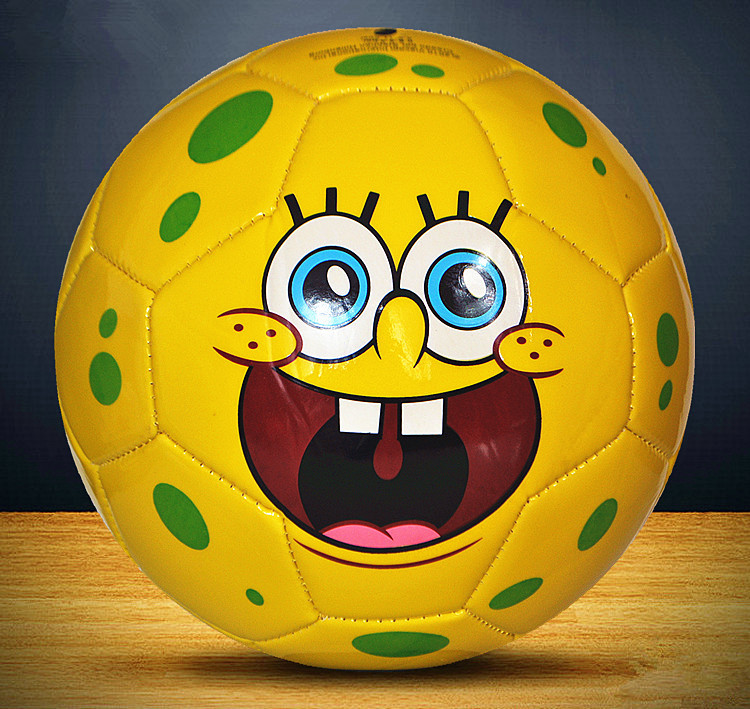
\includegraphics[scale=0.09]{ibagens/ball.jpg}
\source{A internet}
\end{figure}
\end{lstlisting}
\ownsrc
\end{figure}
\vspace{-0.5cm}
\begin{figure}[!h]
\centering
\caption{Uma bola}
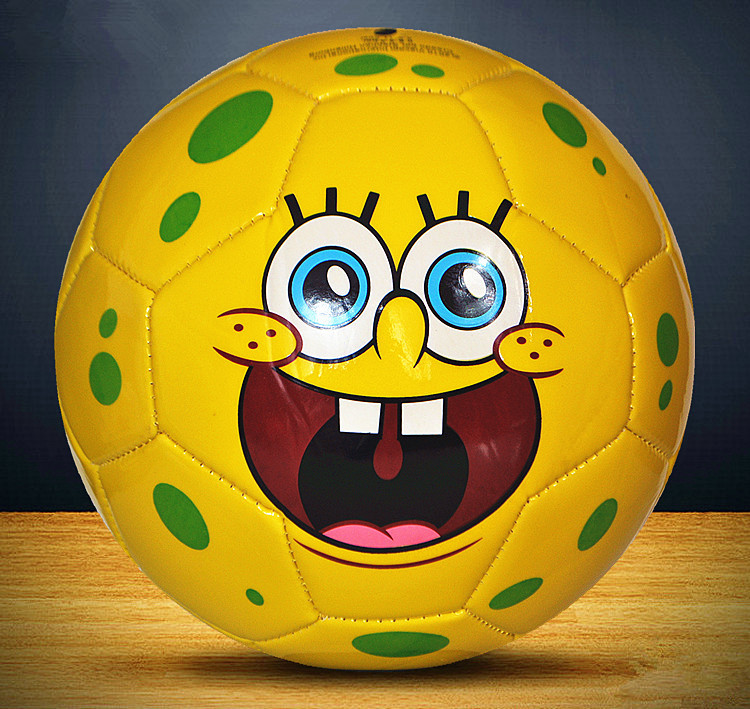
\includegraphics[scale=0.09]{ibagens/ball.jpg}
\\ \small{Fonte: A internet}
\end{figure}
\end{frame}

\begin{frame}[fragile] \frametitle{O ambiente \texttt{figure}}
\vspace{-0.5cm}
\begin{figure}[!t]
\caption{Exemplo de figura}
\begin{lstlisting}
@*\sel{\textbackslash{}begin\{figure\}[!h]}*@
\centering
\caption{Uma bola}
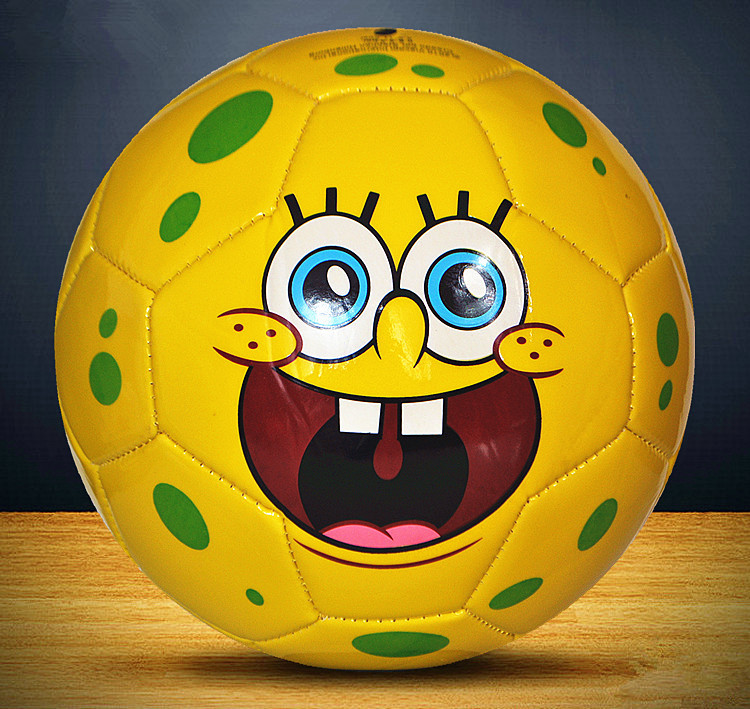
\includegraphics[scale=0.09]{ibagens/ball.jpg}
\source{A internet}
@*\sel{\textbackslash{}end\{figure\}[!h]}*@
\end{lstlisting}
\ownsrc
\end{figure}

\begin{itemize}
	\item \sel{\textbackslash{}begin\{figure\}} e \sel{\textbackslash{}end\{figure\}}
	\begin{itemize}
		\item Define um ambiente de tabela
		\item Pode ter como argumento opcional o \textbf{posicionamento} do \textit{float} dentro do documento\footnote{Ver Tabela~\ref{tab:posicaofloats}}
	\end{itemize}
\end{itemize}
\end{frame}

\begin{frame}[fragile] \frametitle{O ambiente \texttt{figure}}
\vspace{-0.5cm}
\begin{figure}[!t]
\caption{Exemplo de figura}
\begin{lstlisting}
\begin{figure}[!h]
@*\sel{\textbackslash{}centering}*@
@*\seli{\textbackslash{}caption\{Uma bola\}}*@
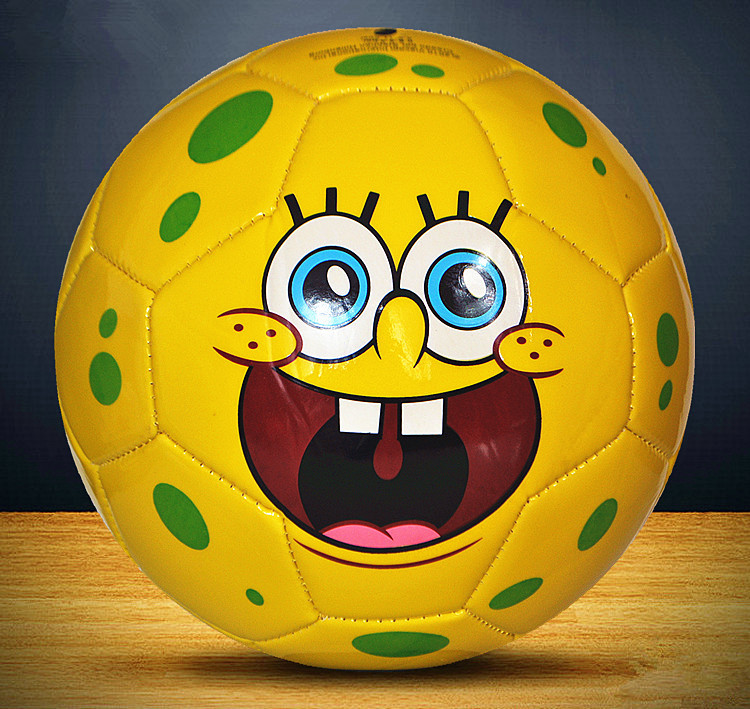
\includegraphics[scale=0.09]{ibagens/ball.jpg}
@*\selii{\textbackslash{}source\{A internet\}}*@
\end{figure}
\end{lstlisting}
\ownsrc
\end{figure}

\begin{itemize}
	\item \sel{\textbackslash{}centering}\footnote{Ver slide~\ref{slide:floatcentering}}, \seli{\textbackslash{}caption\{legenda\}}\footnote{Ver slide~\ref{slide:floatcaptionsource}} e \selii{\textbackslash{}source\{fonte\}}\footnote{Ver slides~\ref{slide:floatcaptionsource} e~\ref{slide:floatjustsource}}
	\begin{itemize}
		\item Elementos comuns a \textit{floats}, como visto nas tabelas
	\end{itemize}
\end{itemize}
\end{frame}

\begin{frame}[fragile] \frametitle{Inclusão de imagens}
\vspace{-0.5cm}
\begin{figure}[!t]
\caption{Exemplo de figura}
\begin{lstlisting}
\begin{figure}[!h]
\centering
\caption{Uma bola}
@*\sel{\textbackslash{}includegraphics[scale=0.09]\{ibagens/ball.jpg\}}*@
\source{A internet}
\end{figure}
\end{lstlisting}
\ownsrc
\end{figure}

\begin{itemize}
	\item \sel{\textbackslash{}includegraphics[opcional]\{arquivo\}}
	\begin{itemize}
		\item Faz a inclusão de um arquivo de imagem externo ao Latex
		\item Em \texttt{arquivo} é passado o caminho onde está a imagem que deseja-se mostrar no documento
		\begin{itemize}
			\item Formatos aceitos: \texttt{pdf}, \texttt{png} e \texttt{jpg}
			\item Para aceitar outros formatos, somente com pacotes adicionais
		\end{itemize}
	\end{itemize}
\end{itemize}
\end{frame}

\begin{frame}[fragile] \frametitle{Inclusão de imagens}
\vspace{-0.5cm}
\begin{figure}[!t]
\caption{Exemplo de figura}
\begin{lstlisting}
\begin{figure}[!h]
\centering
\caption{Uma bola}
@*\sel{\textbackslash{}includegraphics[scale=0.09]\{ibagens/ball.jpg\}}*@
\source{A internet}
\end{figure}
\end{lstlisting}
\ownsrc
\end{figure}

\begin{itemize}
	\item \sel{\textbackslash{}includegraphics[opcional]\{arquivo\}}
	\begin{itemize}
		\item Em \texttt{opcional} podem ser passados alguns argumentos optativos, sendo os mais utilizados:
		\begin{itemize}
			\item \texttt{scale=escala}, onde fazemos o redimensionamento da imagem
			\item \texttt{width=valor}, onde limitamos a largura da imagem
			\item Dentre outros
		\end{itemize}
	\end{itemize}
\end{itemize}
\end{frame}

%\usepackage{graphicx}
\begin{frame}[fragile] \frametitle{Inclusão de imagens}
\vspace{-0.5cm}
\begin{figure}[!t]
\caption{Exemplo de figura}
\begin{lstlisting}
@*\seli{\textbackslash{}usepackage\{graphicx\}}*@
(@*\ldots*@)
\begin{document}
(@*\ldots*@)
\begin{figure}[!h]
\centering
\caption{Uma bola}
@*\sel{\textbackslash{}includegraphics[scale=0.09]\{ibagens/ball.jpg\}}*@
\source{A internet}
\end{figure}
\end{lstlisting}
\ownsrc
\end{figure}

\begin{itemize}
	\item \sel{\textbackslash{}includegraphics[opcional]\{arquivo\}}
	\begin{itemize}
		\item Por padrão, o Latex \textbf{não} tem suporte a este comando
		\item Necessariedade de um pacote
		\begin{itemize}
			\item \texttt{graphicx}
			\item Incluímos no preâmbulo do documento \seli{\textbackslash{}usepackage\{graphicx\}}
		\end{itemize}
	\end{itemize}
\end{itemize}
\end{frame}

\begin{frame}[fragile] \frametitle{Refência a figuras}

\begin{itemize}
	\item Vimos como fazer refência à seções e tabelas
	\item Referencia de figuras = referência de tabelas
\end{itemize}

\end{frame}

\begin{frame}[fragile] \frametitle{Refência a figuras}
\begin{figure}[!t]
\caption{Exemplo de figuras}
\begin{lstlisting}
\begin{figure}[!h]
\centering
\caption{Uma bola}
@*\sel{\textbackslash{}label\{minhaimagem\}}*@
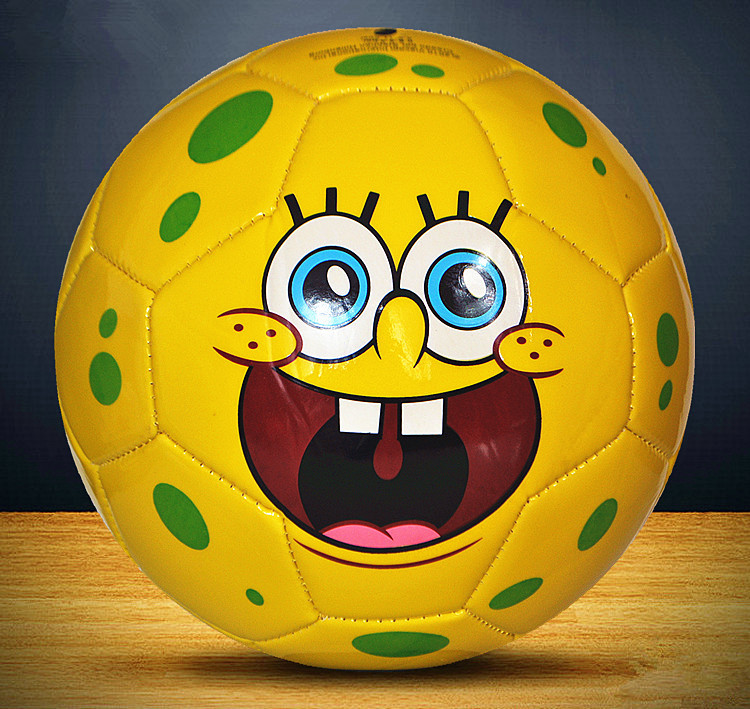
\includegraphics[scale=0.09]{ibagens/ball.jpg}
\source{A internet}
\end{figure}

Na Figura~@*\seli{\textbackslash{}ref\{minhaimagem\}}*@, são mostrados (@*\ldots*@)
\end{lstlisting}
\ownsrc
\end{figure}

\begin{itemize}
	\item Utilizamos o par de comandos \sel{\textbackslash{}label} e \seli{\textbackslash{}ref}, tal qual tabelas\footnote{Ver slide~\ref{slide:referenciatabela}}
\end{itemize}

\end{frame}

%\label{tab:posicaofloats}


% Referências bibliográficas..
\section{Bibliografia}

\begin{frame}[fragile] \frametitle{Bibliografia}
\begin{itemize}
	\item Desenvolvimento de bons trabalhos acadêmicos implicam em boas referências bibliográficas
	\item Latex fornece um esquema de citações e referências bibliográficas
	\begin{itemize}
		\item Nomeia uma referência para depois citá-la
	\end{itemize}
\end{itemize}
\end{frame}

\begin{frame}[fragile] \frametitle{Bibliografia do zero (Estilo)}
\vspace{-0.5cm}
\begin{figure}[!t]
\caption{Bibliografia do zero}
\begin{lstlisting}
@*\sel{\textbackslash{}bibliographystyle\{acm\}}*@
\bibliography{bibliografia.bib}
\end{lstlisting}
\ownsrc
\end{figure}

\begin{itemize}
	\item \sel{\textbackslash{}bibliographystyle\{acm\}}
	\begin{itemize}
		\item Define o estilo de bibliografia a ser utilizado.
		\item O Latex já fornece alguns como padrão
		\begin{itemize}
			\item \texttt{plain}, \texttt{unsrt}, \texttt{abbrv}, \texttt{alpha}, \ldots
		\end{itemize}
	\end{itemize}
\end{itemize}
\end{frame}

\begin{frame}[fragile] \frametitle{Bibliografia do zero (Estilo)}
\vspace{-0.5cm}
\begin{figure}[!t]
\caption{Bibliografia do zero}
\begin{lstlisting}
@*\sel{\textbackslash{}bibliographystyle\{acm\}}*@
\bibliography{bibliografia.bib}
\end{lstlisting}
\ownsrc
\end{figure}

\begin{itemize}
	\item \sel{\textbackslash{}bibliographystyle\{acm\}}
	\begin{itemize}
		\item Podemos utilizar padrões personalizados
		\item Tal qual existem as classes de documentos, também existem classes para bibliografia
		\begin{itemize}
			\item Comumente fornecidas em arquivos .bst
		\end{itemize}
		\item Classe do TCC do TSI: abnt.bst
	\end{itemize}
\end{itemize}
\end{frame}

\begin{frame}[fragile] \frametitle{Bibliografia do zero}
\vspace{-0.5cm}
\begin{figure}[!t]
\caption{Bibliografia do zero}
\begin{lstlisting}
\bibliographystyle{acm}
@*\sel{\textbackslash{}bibliography\{bibliografia.bib\}}*@
\end{lstlisting}
\ownsrc
\end{figure}

\begin{itemize}
	\item \sel{\textbackslash{}bibliography\{arquivo\}}
	\begin{itemize}
		\item Informa qual o arquivo externo que fornece a bibliografia
		\item Geralmente é atribuido a extensão .bib
		\item Este arquivo segue um formato diferente
		\begin{itemize}
			\item \textbf{Bibtex}
		\end{itemize}
	\end{itemize}
\end{itemize}
\end{frame}

\begin{frame}[fragile] \frametitle{Arquivo .bib}
\vspace{-0.5cm}
\begin{figure}[!t]
\caption{Exemplo de uma entrada no arquivo .bib}
\begin{lstlisting}[language=BibTeX]
@*\sel{@article}*@{rodriguez1985consideraciones,
  title={Consideraciones relativas a la actuaci{\'o}n y l{\'\i}mites de las oposiciones fonol{\'o}gicas interrupto/continuo y tenso/flojo en espa{\~n}ol},
  author={Rodr{\'\i}guez, Alexandre Veiga},
  journal={Verba: Anuario galego de filoloxia},
  number={12},
  pages={253--286},
  year={1985},
  publisher={Servicio de Publicaciones}
}
\end{lstlisting}
\ownsrc
\end{figure}

\begin{itemize}
	\item \sel{@tipo}
	\begin{itemize}
		\item Define o tipo de bibliografia. Se é artigo, livro, \textit{site}, dentre outros
	\end{itemize}
\end{itemize}
\end{frame}

\begin{frame}[fragile] \frametitle{Arquivo .bib (Tipos)}

\begin{itemize}
	\item Existem diversos tipos para uma entrada de bibliografia
	\item Formatos aceitos: 
	\begin{itemize}
		\item @article ,@book ,@collectedbook ,@conference ,@electronic ,@ieeetranbstctl ,@inbook ,@incollectedbook ,@incollection ,@injournal ,@inproceedings ,@manual ,@mastersthesis ,@misc ,@patent ,@periodical ,@phdthesis ,@preamble ,@proceedings ,@standard ,@string ,@techreport e @unpublished
	\end{itemize}
\end{itemize}

\end{frame}

\begin{frame}[fragile] \frametitle{Arquivo .bib}
\vspace{-0.5cm}
\begin{figure}[!t]
\caption{Exemplo de uma entrada no arquivo .bib}
\begin{lstlisting}[language=BibTeX]
@article{@*\sel{rodriguez1985consideraciones}*@,
  title={Consideraciones relativas a la actuación y límites de las oposiciones fonológicas interrupto/continuo y tenso/flojo en español},
  author={Rodríguez, Alexandre Veiga},
  journal={Verba: Anuario galego de filoloxia},
  number={12},
  pages={253--286},
  year={1985},
  publisher={Servicio de Publicaciones}
}
\end{lstlisting}
\ownsrc
\end{figure}

\begin{itemize}
	\item \sel{rótulo da referência}
	\begin{itemize}
		\item Define o rótulo da bibliografia
		\item Importante pois usaremos ela para fazer a referência no texto
		\item Neste caso, o nome é \texttt{rodriguez1985consideraciones}
	\end{itemize}
\end{itemize}

\end{frame}

\begin{frame}[fragile] \frametitle{Arquivo .bib}
\vspace{-0.5cm}
\begin{figure}[!t]
\caption{Exemplo de uma entrada no arquivo .bib}
\begin{lstlisting}[language=BibTeX]
@article{rodriguez1985consideraciones,
  @*\sel{title}*@={Consideraciones relativas a la actuación y límites de las oposiciones fonológicas interrupto/continuo y tenso/flojo en español},
  @*\sel{author}*@={Rodríguez, Alexandre Veiga},
  @*\sel{journal}*@={Verba: Anuario galego de filoloxia},
  @*\sel{number}*@={12},
  @*\sel{pages}*@={253--286},
  @*\sel{year}*@={1985},
  @*\sel{publisher}*@={Servicio de Publicaciones}
}
\end{lstlisting}
\ownsrc
\end{figure}

\begin{itemize}
	\item \sel{campo da referência=\{valor\}}
	\begin{itemize}
		\item Estabelece um campo para a referência, o qual representa alguma informação
		\begin{itemize}
			\item Título, ano de publicação, revista, \ldots
		\end{itemize}
	\end{itemize}
\end{itemize}
\end{frame}

\begin{frame}[fragile] \frametitle{Arquivo .bib (Campos)}
\begin{itemize}
	\item Existem vários campos para uma entrada bibliográfica
	\item Campos aceitos: 
	\begin{itemize}
		\item address, annote, author, booktitle, chapter, crossref, edition, editor, howpublished, institution, journal, key, month, note, number, organization, pages, publisher, school, series, title, type, volume, year
	\end{itemize}
	\item Dependendo do formato de bibliografia utilizado, cada \textbf{tipo} necessita de determinados \textbf{campos}
	\begin{itemize}
		\item O formato fornecido por abnt.bst insere alguns indicadores para caso de falta de informação
	\end{itemize}
\end{itemize}
\end{frame}

\begin{frame}[fragile] \frametitle{Ainda sobre o arquivo .bib}
\begin{itemize}
	\item Caracteres especiais no arquivo .bib
	\begin{itemize}
		\item ã, â, á, à, ç, \ldots
	\end{itemize}
	\item Salvar o arquivo .bib \textbf{no mesmo formato de codificação que o .tex}
	\begin{itemize}
		\item UTF-8 sendo preferível
	\end{itemize}
\end{itemize}
\end{frame}

\begin{frame}[fragile] \frametitle{Ainda sobre o arquivo .bib}
\begin{itemize}
	\item Precisamos construir toda a entrada formatada para todas as referências?
	\begin{itemize}
		\item Não necessariamente
	\end{itemize}
	\item Grande parte das bases de dados de livros, artigos, dentre outros, \textbf{já fornecem a bibliografia em formato Bibtex}
	\begin{itemize}
		\item Google Scholar
		\item IEEE
		\item ACM
	\end{itemize}
	\item Diminui os esforços para a bibliografia
\end{itemize}
\end{frame}

\begin{frame}[fragile] \frametitle{Citação bibliográfica}
\begin{itemize}
	\item Tendo uma entrada no arquivo .bib, podemos fazer a citação da mesma
	\item Voltaremos ao nosso arquivo .tex
\end{itemize}
\end{frame}

\begin{frame}[fragile] \frametitle{Citação bibliográfica}
\vspace{-0.5cm}
\begin{figure}[!t]
\caption{Citação bibliográfica}
\begin{lstlisting}
	Como dito em~@*\sel{\textbackslash{}cite\{rodriguez1985consideraciones\}}*@, existem alguns fatores (@*\ldots*@)
\end{lstlisting}
\ownsrc
\end{figure}

\begin{itemize}
	\item \sel{\textbackslash{}cite\{rótulo da citação\}}
	\begin{itemize}
		\item Faz a citação de uma bibliografia, utilizando um rótulo já definido
		\begin{itemize}
			\item O Latex já se encarrega de referenciar corretamente
			\item Se for o caso, a numeração também fica a cargo do Latex
		\end{itemize}
	\end{itemize}
\end{itemize}
\end{frame}
% Particularidades extras..
\section{Particularidades}

\begin{frame}[fragile] \frametitle{Particularidades}

\begin{itemize}
	\item Adendo à codificação de caracteres
	\item Fontes \texttt{TrueType}
	\item Modularização
\end{itemize}

\end{frame}

\begin{frame}[fragile] \frametitle{Um adendo à codificação de caracteres}
\begin{itemize}
	\item Em alguns casos específicos, não será possível inserir caracteres especiais
	\begin{itemize}
		\item Quando editamos documentos com classes que fornecem diferentes codificações
	\end{itemize}
	\item É possível fazer a inserção de caracteres especiais \textbf{mesmo} em diferentes codificações
	\item Existe comandos para isto
	\begin{itemize}
		\item Em algumas referências prontas do Bibtex é possível verificar tais comandos
	\end{itemize}
\end{itemize}
\end{frame}

\begin{frame}[fragile] \frametitle{Um adendo à codificação de caracteres}
\begin{figure}[!t]
\begin{lstlisting}[language=BibTeX]
@article{rodriguez1985consideraciones},
  title={Consideraciones relativas a la actuaci@*\sel{\textbackslash{}'\{o\}}*@n y l@*\sel{\textbackslash{}'\{i\}}*@mites de las oposiciones fonol@*\sel{\textbackslash{}'\{o\}}*@gicas interrupto/continuo y tenso/flojo en espa@*\sel{\textbackslash{}\textasciitilde{}\{n\}}*@ol},
  (@*\ldots*@)
}
\end{lstlisting}
\end{figure}

\begin{itemize}
	\item \sel{\textbackslash{}adicional\{caractere\}}
	\begin{itemize}
		\item Permite a inserção de um caractere especial
		\item Em \sel{caractere}, descrevemos qual o caractere que levará um "adendo"
		\item Em \sel{adicional}, inserimos o que vai no caractere
		\begin{itemize}
			\item \sel{\textbackslash{}'\{o\}}: Estamos colocando \texttt{'} (que acento agudo) no caractere \texttt{o}
			\item O resultado é o caractere especial \texttt{ó}
		\end{itemize}
	\end{itemize}
\end{itemize}
\end{frame}

\begin{frame}[fragile] \frametitle{Um adendo à codificação de caracteres}
\begin{table}[!t]
\caption{Comandos para inserção de caracteres especiais utilizados em português}
\begin{tabular}{l|l|l} \hline
\textbf{Comando} & \textbf{Saída} & \textbf{Descrição} \\ \hline
\texttt{\textbackslash{}`\{o\}}                  & ò & Acento grave \\ \hline
\texttt{\textbackslash{}'\{o\}}                  & ó & Acento agudo \\ \hline
\texttt{\textbackslash{}\textasciicircum{}\{o\}} & ô & Circunflexo  \\ \hline
\texttt{\textbackslash{}$\sim$\{o\}}             & õ & Til          \\ \hline
\texttt{\textbackslash{}c\{c\}}                  & ç & Cedilha      \\ \hline
\end{tabular}
\end{table}

\begin{itemize}
	\item Lembrete: Embora os exemplos acima na maioria das vezes utilizam \texttt{o} como exemplo, basta trocar o caractere para descrever outros caracteres especiais
	\begin{itemize}
		\item \texttt{\textbackslash{}'\{a\}}: \texttt{á}
	\end{itemize}
\end{itemize}
\end{frame}

\begin{frame}[fragile] \frametitle{Fontes \texttt{TrueType}}
\begin{itemize}
	\item Ao longo destes \textit{slides} foram vistos diversas vezes o uso de fontes \texttt{TrueType}
	\begin{itemize}
		\item Fontes as quais todos os caracteres ocupam o mesmo tamanho!
		\item Fonte ideal para a mostra de \textbf{código}
	\end{itemize}
	\item Simples: \sel{\textbackslash{}texttt\{texto em truetype\}}
\end{itemize}
\end{frame}

\begin{frame}[fragile] \frametitle{Modularização}
\begin{itemize}
	\item Se assim desejarmos, podemos dividir nosso projeto em Latex em vários arquivos
	\begin{itemize}
		\item Interessante quando temos um projeto grande
		\item Duas formas
	\end{itemize}
\end{itemize}
\end{frame}

\begin{frame}[fragile] \frametitle{\texttt{input} vs. \texttt{include}}
\begin{itemize}
	\item \sel{\textbackslash{}input\{nome do arquivo\}}
	\begin{itemize}
		\item Inclui um arquivo externo do tipo .tex
		\item Funcionamento: Tudo que está dentro do arquivo externo é passado para onde houve a chamada do comando \texttt{\textbackslash{}input}
	\end{itemize}
	\item \sel{\textbackslash{}include\{nome do arquivo\}}
	\begin{itemize}
		\item Inclui um arquivo externo do tipo .tex, porém em uma \textbf{nova página}
		\item Funcionamento: É feita uma quebra de página, e então o conteúdo do arquivo externo é passado para onde houve a chamada do comando \texttt{\textbackslash{}include}	
	\end{itemize}
\end{itemize}
\end{frame}
% Outras possibilidades
\section{Outras Possibilidades}

\begin{frame}[fragile] \frametitle{Outras Possibilidades}
\begin{itemize}
	\item Existem \textbf{muitas} possibilidades em Latex
	\begin{itemize}
		\item Comunidade do Latex bem ativa
		\item Desenvolvimento de diversos pacotes para múltiplos fins
	\end{itemize}
\end{itemize}
\end{frame}

\begin{frame}[fragile] \frametitle{Apresentações}
\begin{itemize}
	\item Mudanças na \textbf{classe de documentos}
	\item Alguns comandos adicionais
	\item De restante, \textbf{grande parte} dos comandos em Latex são aplicáveis
	\item Tal qual o \textit{template} do TSI para TCC, existe um formato voltado para apresentações
	\begin{itemize}
		\item Também disponível no github
		\item \url{https://github.com/gdotorres/apresentacao-tsi-pelotas}
	\end{itemize}
\end{itemize}
\end{frame}

\begin{frame}[fragile] \frametitle{Ambiente matemático}
\begin{itemize}
	\item Permite uma ampla variedade de comandos os quais fornecem meios para formatação de conceitos matemáticos
	\begin{itemize}
		\item Equações, fórmulas, \ldots
	\end{itemize}
	\item Utiliza uma série de caracteres especiais, os quais são definidos em uma extensa lista de comandos\footnote{\url{https://en.wikibooks.org/wiki/LaTeX/Mathematics\#List\_of\_mathematical\_symbols}}
	\item Possível construir equação em um ambiente online, permitindo mais rapidez e geração automática do código
	\begin{itemize}
		\item Online LaTeX Equation Editor: \url{https://www.codecogs.com/eqnedit.php}
	\end{itemize}
\end{itemize}
\end{frame}

\begin{frame}[fragile] \frametitle{Outras funcionalidades}
\begin{itemize}
	\item Desenho de figuras
	\item Gráficos
	\item Códigos
	\item Diversos
\end{itemize}
\end{frame}




\end{document} 

